% =====================================================================
%  Paper From Zero Guide -- LaTeX template
%  Copy this file, replace every <<...>> placeholder, keep the preamble.
%  Compile 3 times: pdflatex -interaction=nonstopmode guide.tex
% =====================================================================
\documentclass[11pt,a4paper]{article}
\usepackage[margin=2cm,headheight=14pt]{geometry}
\usepackage[T1]{fontenc}
\usepackage[scaled=0.95]{helvet}
\renewcommand{\familydefault}{\sfdefault}
\usepackage{amsmath,amssymb,bm,mathtools}
\usepackage[table]{xcolor}
\usepackage[most]{tcolorbox}
\usepackage{tikz}
\usetikzlibrary{arrows.meta,positioning,shapes.geometric,calc,fit,backgrounds,decorations.pathreplacing,decorations.pathmorphing}
\usepackage{booktabs,tabularx,xltabular,array,enumitem,titlesec,fancyhdr,float,caption,needspace,graphicx}
\usepackage{annotate-equations}
\usepackage[hidelinks]{hyperref}

% ---------- colors ----------
\definecolor{navy}{HTML}{1B3A5C}
\definecolor{teal}{HTML}{00798C}
\definecolor{rosered}{HTML}{D1495B}
\definecolor{amber}{HTML}{E09F3E}
\definecolor{leaf}{HTML}{2E8B57}
\definecolor{plum}{HTML}{6A4C93}

% ---------- labeled equations ----------
\renewcommand{\eqnhighlightheight}{\mathstrut}
\renewcommand{\eqnannotationfont}{\bfseries\small}

% ---------- boxes ----------
\newtcolorbox{eqbox}[1]{enhanced,breakable,colback=white,colframe=navy,boxrule=0.9pt,arc=2mm,title={#1},fonttitle=\bfseries,coltitle=white,colbacktitle=navy}
\newtcolorbox{verdict}[1]{enhanced,breakable,colback=teal!6,colframe=teal,boxrule=0.9pt,arc=2mm,title={#1},fonttitle=\bfseries}
\newtcolorbox{goodbox}[1]{enhanced,breakable,colback=leaf!6,colframe=leaf,boxrule=0.9pt,arc=2mm,title={#1},fonttitle=\bfseries}
\newtcolorbox{notebox}[1]{enhanced,breakable,colback=amber!8,colframe=amber,boxrule=0.9pt,arc=2mm,title={#1},fonttitle=\bfseries,coltitle=black}
\newtcolorbox{proofbox}[1]{enhanced,breakable,colback=plum!5,colframe=plum,boxrule=0.9pt,arc=2mm,title={#1},fonttitle=\bfseries}
\newtcolorbox{zerobox}[1]{enhanced,breakable,colback=rosered!5,colframe=rosered,boxrule=0.9pt,arc=2mm,title={#1},fonttitle=\bfseries}

% ---------- tables ----------
\newcolumntype{P}[1]{>{\raggedright\arraybackslash}p{#1}}
\newcolumntype{Y}{>{\raggedright\arraybackslash}X}

% ---------- titles, header, footer ----------
\titleformat{\section}{\color{navy}\Large\bfseries}{\thesection}{0.6em}{}[{\color{teal}\titlerule[1.2pt]}]
\titleformat{\subsection}{\color{teal}\large\bfseries}{\thesubsection}{0.6em}{}
\titleformat{\part}[display]{\centering\color{navy}\Huge\bfseries}{\partname~\thepart}{0.4em}{}[{\color{teal}\titlerule[2pt]}]
\renewcommand{\thepart}{\Alph{part}}
\pagestyle{fancy}\fancyhf{}
\fancyhead[L]{\small\color{navy}<<Short paper title>>}
\fancyhead[R]{\small\color{teal}Guide from zero -- v1}
\fancyfoot[C]{\thepage}
\renewcommand{\headrulewidth}{0.4pt}

\setlist{itemsep=2pt,topsep=3pt}
\newcommand{\qed}{\hfill$\blacksquare$}
\newcommand{\ex}{\textit{Example}}
\setlength{\parindent}{0pt}\setlength{\parskip}{4pt}

\begin{document}
% ==================== COVER ====================
\thispagestyle{empty}
\begin{tikzpicture}[remember picture,overlay]
\fill[navy] (current page.north west) rectangle ([yshift=-8.2cm]current page.north east);
\fill[teal] ([yshift=-8.2cm]current page.north west) rectangle ([yshift=-8.5cm]current page.north east);
\node[anchor=north west,text=white,font=\Huge\bfseries] at ([xshift=2cm,yshift=-1.5cm]current page.north west) {Understanding the Paper from Zero};
\node[anchor=north west,text=white,text width=17cm,font=\Large] at ([xshift=2cm,yshift=-2.9cm]current page.north west) {<<Full paper title>>};
\node[anchor=north west,text=amber!60,text width=17cm] at ([xshift=2cm,yshift=-4.8cm]current page.north west) {<<Authors>>};
\node[anchor=north west,text=white,font=\small] at ([xshift=2cm,yshift=-6.2cm]current page.north west) {Guide version v1 \quad$\cdot$\quad <<date>>};
\end{tikzpicture}
\vspace*{7.2cm}

\begin{verdict}{The whole paper in five sentences}
\begin{enumerate}[leftmargin=1.4em]
\item <<problem>> \item <<difficulty>> \item <<idea>> \item <<how it works>> \item <<main result and limits>>
\end{enumerate}
\end{verdict}

\begin{notebox}{How to read this guide}
Numbers quoted from the paper are exact. Numbers marked \ex{} come from our own code (seed and parameters given). Values marked ``read from figure'' are read by eye from the paper's plots.
\end{notebox}

\begin{center}
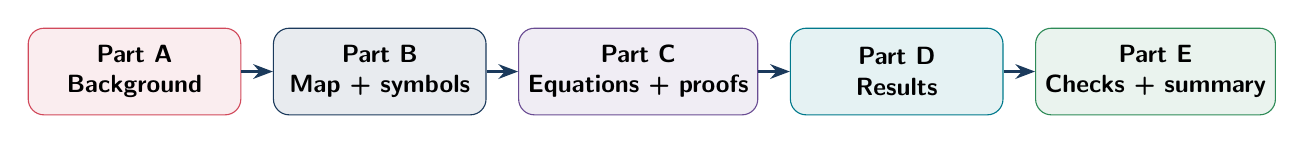
\begin{tikzpicture}[node distance=4mm,b/.style={draw=#1,fill=#1!10,rounded corners=2mm,minimum width=27mm,minimum height=11mm,align=center,font=\small\bfseries}]
\node[b=rosered] (A) {Part A\\Background};
\node[b=navy,right=of A] (B) {Part B\\Map + symbols};
\node[b=plum,right=of B] (C) {Part C\\Equations + proofs};
\node[b=teal,right=of C] (D) {Part D\\Results};
\node[b=leaf,right=of D] (E) {Part E\\Checks + summary};
\foreach \x/\y in {A/B,B/C,C/D,D/E} \draw[-{Stealth[length=2.5mm]},thick,navy] (\x)--(\y);
\end{tikzpicture}
\end{center}
\newpage
\tableofcontents
\clearpage

% ==================== PART A ====================
\part{Background from zero}
\Needspace{14\baselineskip}
\section{<<First concept>>}
<<Short sentences, simple words.>>
\begin{zerobox}{Everyday analogy}
<<analogy>>
\end{zerobox}

% ==================== PART B ====================
\clearpage
\part{Map and symbols}
\Needspace{14\baselineskip}
\section{The equation map}
\begin{center}
\def\dx{40mm}\def\dy{25mm}
\begin{tikzpicture}[n/.style={draw=#1,fill=#1!10,rounded corners=2mm,text width=29mm,minimum height=13mm,align=center,font=\footnotesize},
 ar/.style={-{Stealth[length=2.5mm]},thick,navy}, lb/.style={font=\scriptsize,fill=white,inner sep=1pt}]
\node[n=navy] (e1) at (0,0) {\textbf{Eq.~(1)}\\model};
\node[n=plum] (e2) at (\dx,0) {\textbf{Eq.~(2)}\\estimator};
\node[n=rosered] (e3) at (2*\dx,0) {\textbf{Eq.~(3)}\\decision};
\draw[ar] (e1)--node[lb,above]{input}(e2);
\draw[ar] (e2)--node[lb,above]{score}(e3);
\end{tikzpicture}
\end{center}

% ==================== PART C ====================
\clearpage
\part{Every equation, with proofs}
\Needspace{14\baselineskip}
\section{Eq.~(1): <<name>>}
% Mark names must be unique in the whole document (prefix per box: qA..., qB...).
% Alternate above/below and left/right; stack labels on the same side with yshift 1.2em / 2.6em.
\begin{eqbox}{Equation (1) -- <<short meaning>>}
\vspace*{2.8em}
\begin{equation*}
\eqnmarkbox[navy]{qAy}{y}=\eqnmarkbox[teal]{qAh}{h}\,x+\eqnmarkbox[rosered]{qAn}{n}
\end{equation*}
\annotate[yshift=1.2em]{above,left}{qAy}{what we receive}
\annotate[yshift=-1.2em]{below,left}{qAh}{channel gain}
\annotate[yshift=1.2em]{above,right}{qAn}{noise}
\vspace*{2.6em}
\end{eqbox}

\textbf{In plain words.} <<...>>

\begin{proofbox}{Proof of Eq.~(1)}
\textbf{Conditions.} <<every condition the proof needs>>
\begin{enumerate}[leftmargin=1.4em]
\item <<step>>
\item <<step>> \qed
\end{enumerate}
\end{proofbox}

\begin{goodbox}{Small example with numbers (\ex)}
<<numbers from numbers.json>>
\end{goodbox}
\textbf{Why the paper needs it.} <<...>>

% ==================== PART D ====================
\clearpage
\part{Results explained}
\Needspace{14\baselineskip}
\section{Main table rebuilt}
\begin{center}
\rowcolors{2}{navy!5}{white}
\begin{tabular}{lcc}
\toprule
\textbf{Method} & \textbf{Metric 1} & \textbf{Metric 2}\\\midrule
<<A>> & <<..>> & <<..>>\\
<<B>> & <<..>> & <<..>>\\
\bottomrule
\end{tabular}
\end{center}
\begin{notebox}{What to see}
<<...>>
\end{notebox}

% ==================== PART E ====================
\clearpage
\part{Checks and summary}
\Needspace{14\baselineskip}
\section{Checked by our own simulation}
{\small
\rowcolors{2}{leaf!6}{white}
\begin{tabularx}{\textwidth}{YP{3.6cm}P{3.6cm}P{0.9cm}}
\toprule
\textbf{Item} & \textbf{Paper} & \textbf{Ours} & \textbf{OK}\\\midrule
<<item>> & <<paper value>> & <<our value>> & \checkmark\\
\bottomrule
\end{tabularx}}

\begin{verdict}{Correctness}
<<errors found, or ``no errors found''; list notation points>>
\end{verdict}

\clearpage
\Needspace{14\baselineskip}
\section{Summary table: one line per equation}
% Use tabularx here, NOT xltabular (xltabular at the end of the document can fail).
{\small
\rowcolors{2}{navy!5}{white}
\begin{tabularx}{\textwidth}{P{2.4cm}P{4.6cm}Y}
\toprule
\textbf{Equation} & \textbf{Formula (short)} & \textbf{Role in simple words}\\\midrule
Eq.~(1) & $y=hx+n$ & <<...>>\\
\bottomrule
\end{tabularx}}
\end{document}
